\section{Arquitectura del sistema}\label{section:arquitecturaSistema}
La estructura principal del sistema es una aplicación en la nube denominada
Nube de conductores. Se encarga de hacer llegar los mensajes procedentes de
los ciclistas a los vehículos a motor, y los mensajes enviados por los
vehículos a motor a los ciclistas. Además, filtra los mensajes que han sido
mal formados, monitoriza las posiciones de todos los vehículos en la carretera
y es capaz de predecir cuándo se puede dar la posibilidad de que haya un choque
entre dos vehículos; en cuyo caso avisa a los conductores de esta posibilidad.

Los vehículos a motor se mantienen mandando continuamente beacons a través
de un \gls{obu}. Para enviar los mensajes emplean el canal broadcast de la
red \Gls{802.11p}. En estos mensajes anuncian al resto de vehículos su
posición, velocidad y dirección hacia la que circulan. No se comunican
directamente con la Nube de Conductores, sino que los mensajes enviados
son escuchados por unidades desplegadas en carretera llamada \gls{rsu}.

La \gls{rsu} recibe los mensajes que envían los vehículos y retransmiten esta
información a la Nube de Conductores. Así mismo, retransmiten los mensajes que
reciben de la nube a los vehículos en carretera; a excepción de que el
destinatario sea la propia \gls{rsu}.

Por otro lado, los ciclistas envían información a la Nube de Conductores a
través de redes móviles; dependiendo de la disponibilidad, \gls{3g} o \gls{lte}.
Éstos también pueden agruparse empleando la red Wi-Fi 802.11, mediante la
creación de un hub para dispositivos móviles en el cual se envían
notificaciones sobre los eventos que aparezcan.

En la Figura \ref{fig:ArquitecturaSistema} se puede observar de qué elementos
está compuesto el sistema y cómo se comunican entre ellos. Como puede
apreciarse, hay diferentes tecnologías de comunicación y desarrollo en cada
una de las plataformas, por lo que uno de los requisitos es que la solución
desarrollada sea flexible a los cambios de tecnología tanto comunicación como
desarrollo.

\begin{figure}[H]
	\begin{center}
		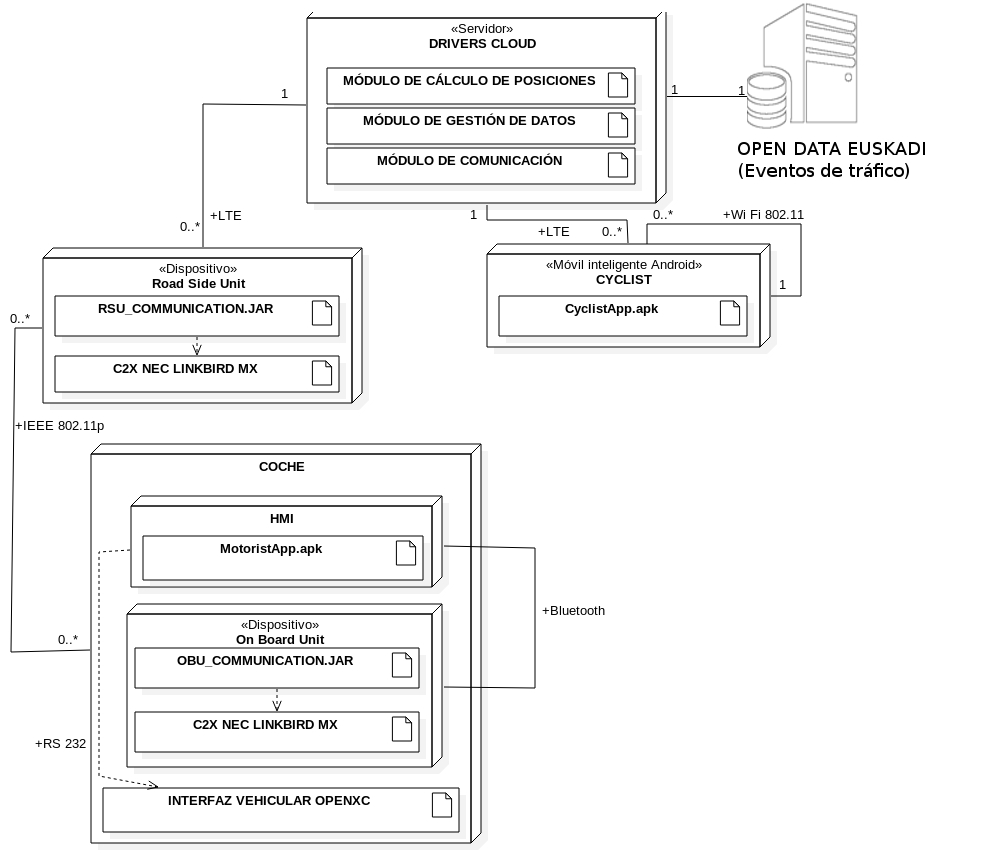
\includegraphics[scale=0.4]{arquitectura_global}
		\caption{Arquitectura del sistema}
		\label{fig:ArquitecturaSistema}
	 \end{center}
\end{figure}

\subsection{Comunicación entre plataformas}\label{ssection:comunicacion_plataformas}
La conexión entre la parte de los vehículos a motor y de los ciclistas hacia la
nube se establece a través de tecnología móvil \gls{lte} o \gls{3g},
dependiendo de la disponibilidad, aunque la manera de comunicarse con la Nube
de Conductores es diferente. La nube actúa como intermediario entre las
aplicaciones desarrolladas en el lado de los motoristas (Sección
\ref{section:comunicacion_vehicular}) y el de los ciclistas (Sección
\ref{section:appCiclistas}).

\subsubsection{Mensajes a ciclistas}\label{sssection:mensajes_ciclistas}
Gracias al actual predominio de smartphones en la vida de todos los habitantes,
el despliegue de aplicaciones móviles vehiculares es bastante sencillo. Se han
convertido en dispositivos potentes y versátiles, los cuales permiten
utilizarlos para una gran variedad de utilidades. Gracias a que tienen
el sistema \gls{gps} integrado se puede obtener una posición bastante
aproximada de los usuarios, dependiendo de la calidad del dispositivo se
obtendrá una localización más precisa. También poseen conexión móvil con una
gran variedad de conexiones como Bluetooth, \gls{usb}, Wi-Fi, \gls{lte},
\gls{gsm}, \gls{umts} y \gls{nfc}.

Actualmente el predomino del mercado se encuentra en el Sistema Operativo móvil
Android. Este sistema, actualmente en desarrollo por Google, esta orientado
principalmente a dispositivos móviles y embebidos. Está basado en Linux, y es
un proyecto que tiene devoción por los estándares abiertos existentes; prueba
de ello es la pertenencia a la alianza comercial Open Handset Alliance, la cual
se dedica a desarrollar estándares abiertos para su uso en dispositivos móviles.

Android posee un completo entorno de desarrollo, el cual incluye un depurador
de código, biblioteca, un simulador de teléfono, documentación, ejemplos de
código y tutoriales. Para el desarrollo en esta plataforma se puede optar por
dos opciones, la instalación del \gls{ide} de desarrollo Android Studio, ó
descargar el \gls{sdk} de Android e integrarlo con el IDE que se desee. Los
lenguajes de programación con los que es posible desarrollar son Java y C/C++,
aunque este segundo solo se recomienda su uso para el desarrollo de librerías
que requieran de un gran rendimiento. La aplicación resultante es un paquete
\emph{apk} que es ejecutado dentro de un \emph{sandbox} en Android.

Se ha desarrollado una aplicación Android desde la cual se mandan mensajes
a la nube sobre la posición del usuario o el grupo que el usuario haya
creado. La aplicación recibe notificaciones sobre las posiciones de los
vehículos próximos, y otros diferentes eventos que pueden darse en la
carretera; por ejemplo, un accidente de tráfico. Se ha contemplado la
posibilidad de salidas en grupo de ciclistas, para ello se ha habilitado una
modalidad específica mediante la cual se crea un grupo que se comunica entre
sus miembros a través de una red privada Wi-Fi 802.11. Los miembros se
mantienen actualizados entre ellos sobre los diferentes eventos a través de un
nodo denominado líder, el cual es el enlace a la nube tanto para reportar la
posición del grupo de ciclistas como para recibir mensajes de la nube y
retransmitir éstos al resto de miembros.

Para comunicarse con los dispositivos Android se requiere un sistema de
comunicación por el cual aunque los ciclistas no tengan en un momento
determinado cobertura, los mensajes no se pierdan. Se ha elegido la plataforma
\gls{gcm}, la cual se encarga de gestionar que los mensajes lleguen al destino
aunque éste se encuentre temporalmente inaccesible mediante notificaciones
\emph{Push} [\ref{alg:gcmFuncionamientoMensajes}].

El mensaje debe respetar el formato que la \gls{api} de \gls{gcm} indica y
puede observarse en el algoritmo \ref{alg:gcmformato}, donde \emph{ID\_ANDROID}
es el identificador del dispositivo Android al que se le va a enviar el
mensaje, y \emph{DATOS} un objeto \gls{json} con la información se que desea
enviar. Para crear un identificador único, se puede emplear el que crea Android
cuando se introduce la cuenta de correo personal en el móvil. Un identificador
de Android está formada por una cadena hexadecimal de 64 bits, la cual es poco
probable que se repita. En el caso de que se quisiese reducir aún más la
probabilidad de repetición, se puede mezclar el identificador de Android con
el que la compañía de telefonía emplea para identificar nuestro dispositivo;
aunque esto último aumenta el tamaño de los mensajes.

\begin{listing}
	\begin{minipage}{.4\textwidth}
		\begin{minted}[linenos=true]{java}
{ "registration_ids": [ "ID_ANDROID" ], data: { /*DATOS*/ }}
		\end{minted}
	\end{minipage}
	\caption{Envío de mensajes mediante \gls{gcm}}\label{alg:gcmformato}
\end{listing}

Cuando se inicia una salida, cada vez que el ciclista recibe una posición
actualizada y fiable del \gls{gps}, envía un mensaje a la
Nube de Conductores. La nube actualiza la última posición conocida del
ciclista, y busca vehículos cercanos al ciclista. Si se encuentra algún
resultado, se responde al ciclista con las posiciones de los vehículos que
tiene cercanos. Así mismo, si se detecta que los vehículos están muy cerca, se
envía una alerta al ciclista y al vehículo, de esta forma se les avisa de que
puede haber un adelantamiento entre los dos vehículos (Figura
\ref{fig:DiagSecuencia-Ciclista_Cloud}).

\begin{figure}[h]
	\begin{center}
		\rotatebox{90}{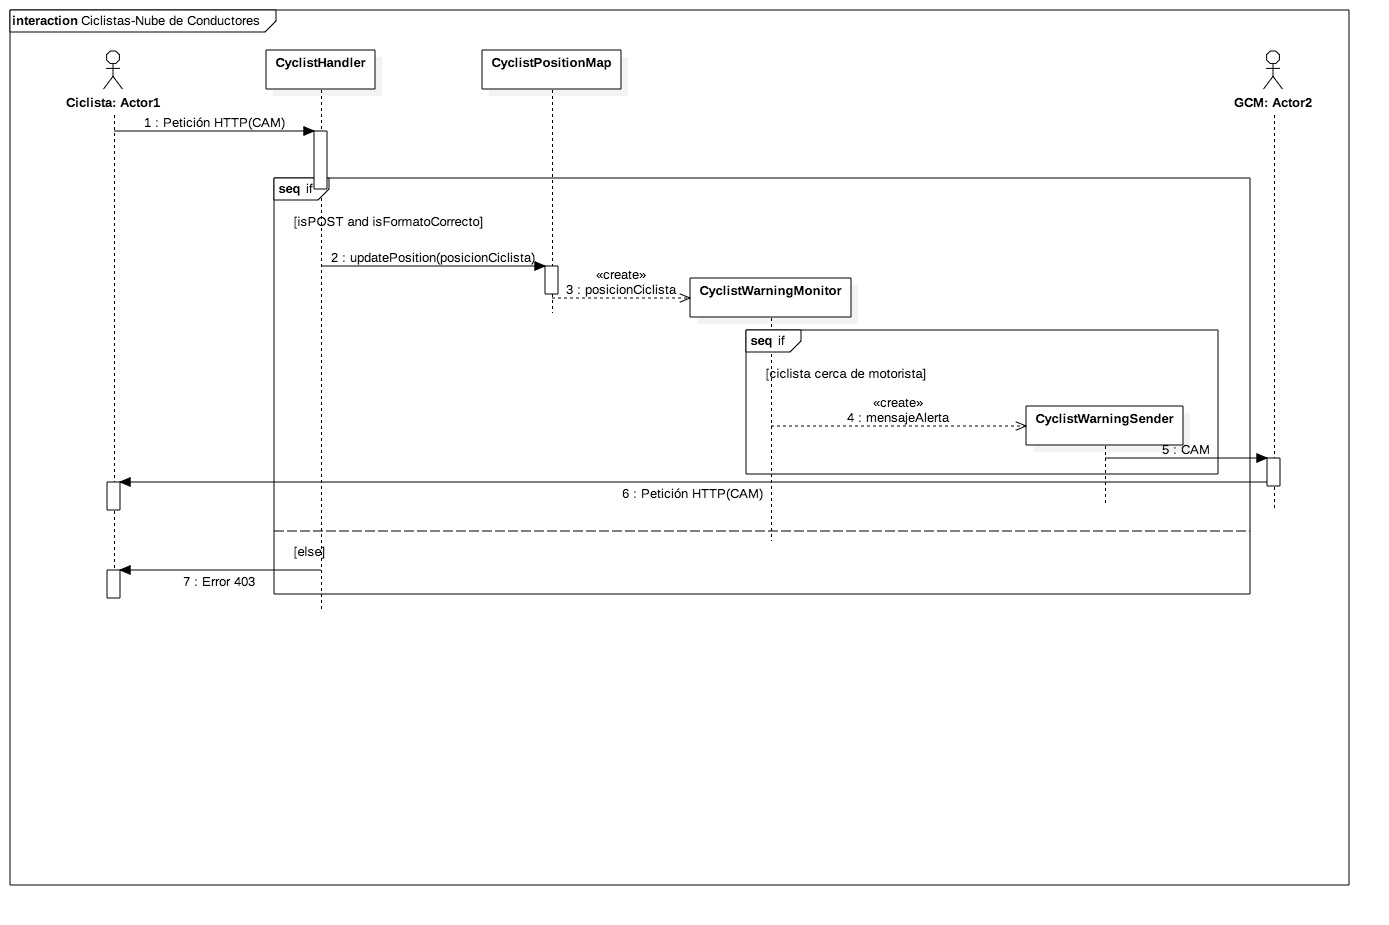
\includegraphics[scale=0.45]{DiagSecuencia-Ciclistas_Cloud}}
		\caption{Ejecución entre Ciclista y la Nube}
		\label{fig:DiagSecuencia-Ciclista_Cloud}
	\end{center}
\end{figure}

\subsubsection{Mensajes a vehículos a motor}\label{sssection:mensajesvehiculomotor}
Los vehículos poseen un dispositivo \gls{obu} que permite comunicarse con la
infraestructura en carretera a través de una red \gls{802.11p}. Gracias a las
\gls{rsu} dispuestas en la carretera, las cuales actúan de intermediario, se
envían y reciben los mensajes de la nube. Esto es posible gracias a la
implementación de servlets que escuchan mensajes provenientes por el puerto
$8080$. Por tanto puede decirse, que las \gls{rsu} actúan de \emph{gateway}
de comunicaciones entre los vehículos y las aplicaciones desplegadas en la
Nube de Conductores. La \gls{obu} al recibir el mensaje lo muestra en un
\emph{HMI} que posee el vehículo. La información del vehículo puede ser
recogida a través de un interfaz OpenXC y/o la \gls{obu}, dependiendo
de la tecnología que se emplee para ello.

En la Figura \ref{fig:DiagSecuencia-OBU_Cloud} se muestra cómo actúan los
componentes cuando un vehículo envía una posición. El \gls{obu} envía una
posición a través del canal broadcast de la red vehicular, cuando un \gls{rsu}
escucha este mensaje, lo redirige inmediatamente a la nube. Una vez en la nube
se actualiza la posición del vehículo, o se añade si no existiese.
Seguidamente, se comprueba si existe un ciclista cercano, si existiese, se
envía las posiciones de los ciclistas encontrados al \gls{rsu}, el cual
redirige al vehículo el mensaje. De poder producirse un adelantamiento o cruce,
se envía una notificación a ambos vehículos.

Los mensajes enviados a los vehículos a motor siguen el formato mostrado en
la sección \ref{ssection:FormatoMensajesNC}. La Nube de Conductores envía
mensajes \Gls{http/1.1} a través del método \emph{post} un mensaje con
contenido \gls{json} a la \gls{rsu}. Ésta se encarga de reenviarlo al vehículo
a través de la red \Gls{802.11p}.

\begin{figure}[h]
	\begin{center}
		\rotatebox{90}{	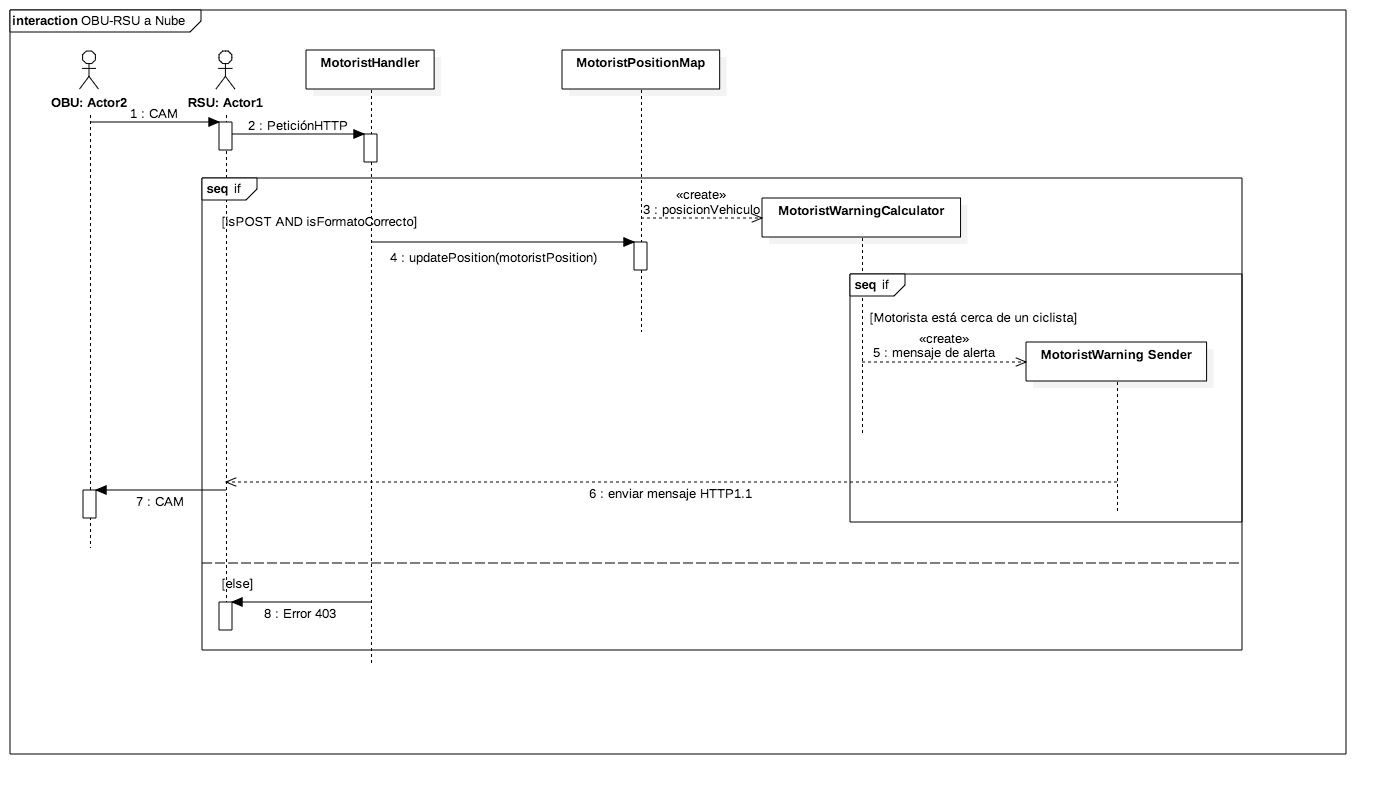
\includegraphics[scale=0.45]{DiagSecuencia-OBU_Cloud} }
		\caption{Ejecución entre \gls{obu}, \gls{rsu} y la Nube de conductores}
		\label{fig:DiagSecuencia-OBU_Cloud}
	\end{center}
\end{figure}
\FloatBarrier

\subsection{Formato de los mensajes}\label{ssection:FormatoMensajesNC}
Para poder realizar la conexión desde diferentes plataformas y entornos de desarrollo,
se ha optado por buscar el diseño más abierto y flexible posible. Los datos son almacenados
y transmitidos en formato plano con la codificación de caracteres \emph{UTF-8}, para
que puedan ser manipulados desde cualquier plataforma. Estos mensajes están construidos
en formato \gls{json} para facilitar su análisis. En el algoritmo \ref{alg:formatoMensajes} se 
muestra un ejemplo de la forma que tienen los mensajes recibidos de vehículos a motor.

\begin{listing}
	\begin{minipage}{.4\textwidth}
		\begin{minted}[linenos=true]{java}
{ "type": "motorist_position", "id": "a3553743", "timestamp": "12343242344",
"latitude": "43.270880", "longitude": "-2.937973", "altitude": "20",
"heading": "53", "speed": "5" }
		\end{minted}
	\end{minipage}
	\caption{Formato de mensajes}\label{alg:formatoMensajes}
\end{listing}

En las siguientes secciones se explica en detalle el formato de los mensajes que
son enviados y recibidos a través de la \emph{Nube de Conductores}.

\subsubsection{Mensaje de posición de vehículo a motor}\label{sssection:MensajePosVehMotor}
Indican la información geográfica de un vehículo. Los mensajes entrantes en la
\emph{Nube de Conductores} tienen que tener todos los campos indicados, mientras
que los mensajes salientes se usarán los campos que sean necesarios. En la
\ref{tab:CamposMensajePosVehMotNubeConductores} se muestra el formato que
deben seguir los mensajes.

\begin{table}[H]
	\centering
	\caption{Formato de mensaje Vehículo a Motor}\label{tab:CamposMensajePosVehMotNubeConductores}
	\begin{tabular}{lll}
		\toprule
			\textbf{Tipo} & \emph{Uso} & \emph{Descripción}\\
		\midrule
			type		&	String	&	Identificador del tipo de mensaje. Su valor es \emph{motorist\_position}.	\\
			id		&	String	&	Identificador del vehículo. Se emplea el ID del router Linkbird-MX		\\
			timestamp	&	Integer	&	Marca de fecha y hora a la que se envía el mensaje.					\\
			latitude	&	Double	&	Latitud en la que se encuentra el vehículo. 						\\
			longitude	&	Double	&	Longitud en la que se encuentra el vehículo.						\\
			altitude	&	Integer	&	Altitud en la que se encuentra el vehículo.						\\
			heading	&	Float		&	Dirección que mantiene el vehículo respecto al Norte magnético.		\\
			speed	&	Float		&	Velocidad a la que circula el vehículo.							\\
		\bottomrule
	\end{tabular}
\end{table}

\subsubsection{Mensaje de posición de ciclista}\label{sssection:MensajePosCiclista}
Indican la información geográfica de uno o más ciclistas. Los mensajes entrantes
en la \emph{Nube de Conductores} tienen que tener todos los campos indicados, mientras
que los mensajes salientes se usarán los campos que sean necesarios [Tabla 
\ref{tab:CamposMensajePosCiclistaNubeConductores}].

\begin{table}[H]
	\centering
	\caption{Formato de mensaje Ciclista}\label{tab:CamposMensajePosCiclistaNubeConductores}
	\begin{tabular}{lll}
		\toprule
			\textbf{Tipo} & \emph{Uso} & \emph{Descripción}\\
		\midrule
			type			&	String	&	Identificador del tipo de mensaje. Su valor es \emph{cyclist\_position}.	\\
			id			&	String	&	Identificador del vehículo. Se emplea el identificador de Android.		\\
			timestamp		&	Integer	&	Marca de fecha y hora a la que se envía el mensaje.					\\
			latitude		&	Double	&	Latitud en la que se encuentra el vehículo. 						\\
			longitude		&	Double	&	Longitud en la que se encuentra el vehículo.						\\
			altitude		&	Integer	&	Altitud en la que se encuentra el vehículo.						\\
			heading		&	Float		&	Dirección que mantiene el vehículo respecto al Norte magnético.		\\
			speed		&	Float		&	Velocidad a la que circula el vehículo.							\\
			components 	&	Integer	&	Número de ciclistas sobre los que se informa.	Permite la creación de
				grupos de ciclistas. 																	\\
		\bottomrule
	\end{tabular}
\end{table}

\subsubsection{Mensaje de alerta}\label{sssection:MensajeAlerta}
Cuando la \emph{Nube de Conductores} detecta que un ciclista y un vehículo a motor
tienen una gran probabilidad de encontrarse, se envía este tipo de mensaje para
comunicar la distancia entre los vehículos y su posición relativa [Apéndice \ref{apendice:posicion_relative}].
Los datos que pueden se incluirse en el mensaje se muestran en la tabla \ref{tab:CamposMensajePosCiclistaNubeConductores}.

\begin{table}[H]
	\centering
	\caption{Formato de mensaje Ciclista}\label{tab:CamposMensajePosCiclistaNubeConductores}
	\begin{tabular}{lll}
		\toprule
			\textbf{Tipo} & \emph{Uso} & \emph{Descripción}\\
		\midrule
			type			&	String	&	Identificador del tipo de mensaje. Su valor es \emph{alert}.	\\
			distance		&	String	&	Distancia a la que se encuentra un vehículo.				\\
			relative\_angle	&	Integer	&	\'Angulo relativo al que se encuentra el vehículo.			\\
		\bottomrule
	\end{tabular}
\end{table}

